% Báo cáo bài tập lớn - Nhóm 09 - Đề 10: Đặt camera giám sát giao thông (Set Cover)
% Biên dịch bằng XeLaTeX: xelatex bao_cao_nhom09_de10.tex (chạy 2 lần để có mục lục).
% Mọi chỗ chữ ĐỎ dạng [ĐIỀN ...] là chỗ nhóm phải bổ sung số liệu/thông tin thật.
% Các hình nằm trong thư mục figures/ (cùng cấp với tệp này).
% Bảng/hình thực nghiệm được sinh từ results/raw/*.csv bằng experiments/shared/summarize.py (bảng nằm ở report/gen/).
\documentclass[a4paper,12pt]{article}
\usepackage{fontspec}
\setmainfont{Liberation Serif}
\setmonofont[Scale=0.85]{DejaVu Sans Mono}
\usepackage[margin=25mm]{geometry}
\usepackage{amsmath,amssymb}
\usepackage{tabularx,booktabs,array,enumitem}
\usepackage{fvextra}
\usepackage{xcolor}
\usepackage{graphicx}
\usepackage[font=small]{caption}
\captionsetup[table]{name=Bảng,labelfont=bf,labelsep=period}
\captionsetup[figure]{name=Hình,labelfont=bf,labelsep=period}
\usepackage{fancyhdr}
\usepackage[hidelinks,unicode]{hyperref}

\setlength{\parindent}{0pt}
\setlength{\parskip}{5pt}
\linespread{1.1}
\emergencystretch=3em
\setlist{itemsep=2pt,topsep=2pt}

\newcolumntype{Y}{>{\raggedright\arraybackslash}X}
\renewcommand{\arraystretch}{1.2}

% Đánh dấu chỗ cần điền
\newcommand{\dien}[1]{\textcolor{red}{[ĐIỀN: #1]}}
\newcommand{\DIEN}{\textcolor{red}{[ĐIỀN]}}

\newcommand{\FriedN}{10}\newcommand{\FriedK}{8}
\newcommand{\FriedChi}{19{,}94}\newcommand{\FriedP}{0{,}0057}
\newcommand{\FriedChiMid}{19{,}94}\newcommand{\FriedPMid}{0{,}0057}
\newcommand{\RankRow}{3{,}20 & 3{,}85 & 4{,}05 & 4{,}90}
\newcommand{\RankRowMid}{3{,}20 & 3{,}85 & 4{,}05 & 4{,}90}

% Khối mã giả
\fvset{fontsize=\footnotesize,breaklines=true,breakanywhere=true,frame=single,framesep=2mm}

\pagestyle{fancy}
\fancyhf{}
\fancyhead[L]{\small Phân tích thiết kế giải thuật}
\fancyhead[R]{\small Nhóm 09 -- Đề 10: Weighted Set Cover}
\fancyfoot[C]{\thepage}
\setlength{\headheight}{15pt}

\begin{document}

%================= TRANG BÌA =================
\begin{titlepage}
\centering
{\Large\bfseries TRƯỜNG ĐẠI HỌC GIAO THÔNG VẬN TẢI\\THÀNH PHỐ HỒ CHÍ MINH\par}
\vspace{0.4cm}{\large Ngành Công nghệ thông tin\par}
\vspace{2.5cm}{\LARGE\bfseries BÁO CÁO BÀI TẬP LỚN\par}
\vspace{0.4cm}{\Large\bfseries HỌC PHẦN: PHÂN TÍCH THIẾT KẾ GIẢI THUẬT\par}
\vspace{1.2cm}{\large\bfseries Đề 10: Đặt camera giám sát giao thông\\
Bài toán phủ tập có trọng số (Weighted Set Cover)\par}
\vspace{1.5cm}
{\bfseries Nhóm 09}\\[4pt]
\begingroup\small\begin{tabular}{llll}
\toprule
Thành viên & Họ tên & MSSV & Phụ trách chính\\
\midrule
A & Phan Việt Anh & 075207008679 & Bộ đọc, bộ kiểm tra, thuật toán chính xác, SA\\
B & Hoàng Duy Khánh & 024207005588 & Tham lam, tìm kiếm cục bộ, TS, bộ sinh dữ liệu\\
C & Huỳnh Xuân Huy & 087205004266 & GA, GA\_LS\\
D & Mai Đàm Công Thành & 038207026777 & GRASP, script thực nghiệm, biểu đồ, thống kê \\
\bottomrule
\end{tabular}\endgroup\\[10pt]
Giảng viên: Nguyễn Văn Huy
\vfill Thành phố Hồ Chí Minh -- Năm học 2026--2027
\end{titlepage}

\renewcommand{\contentsname}{Mục lục}
\tableofcontents
\clearpage

\section*{Tóm tắt}
\addcontentsline{toc}{section}{Tóm tắt}
Báo cáo mô hình hóa việc chọn vị trí đặt camera giám sát giao thông thành bài toán phủ tập có trọng số (NP-khó), cài đặt thuật toán chính xác (nhánh cận kèm giảm cỡ dữ liệu), heuristic tham lam Chvátal, hai chiến lược leo đồi (first/best improvement), bốn metaheuristic (SA, TS, GA, GRASP) và thuật toán lai GA\_LS. Thực nghiệm dùng 10 thể hiện thuộc 3 mức kích thước (4 thể hiện tự sinh nhỏ với $n\le30$, 3 thể hiện tự sinh vừa với $n=400$--$1000$, và 3 thể hiện chuẩn OR-Library \texttt{scp41}, \texttt{scp51}, \texttt{scp61} với $n=1000$--$2000$), mỗi cặp (thuật toán, thể hiện) chạy 10 seed với ngân sách $0{,}5$ s; toàn bộ 800 nghiệm metaheuristic/heuristic (cùng 4 nghiệm EXACT trên bộ nhỏ) đều qua bộ kiểm tra độc lập \texttt{kiemtra.py}.

Kết quả chính: (i) trên 4 thể hiện nhỏ mọi thuật toán trừ tham lam thuần đều tìm được lời giải tối ưu ở 10/10 lần chạy; (ii) trên bộ vừa và OR-Library, các phương pháp kết hợp tìm kiếm cục bộ dẫn đầu: kiểm định Friedman trên 10 thể hiện cho $\chi^2_F=19{,}94$ ($p=0{,}0057$), hạng trung bình tốt nhất thuộc về \texttt{TS} ($3{,}20$), \texttt{GA\_LS} ($3{,}85$) và \texttt{GRASP} ($4{,}05$); \texttt{GRASP} dẫn đầu trên \texttt{vua\_100x400\_s201} ($204{,}00 \pm 0{,}00$) và \texttt{scp41} (best $430$, gap $0{,}23\%$), \texttt{GA\_LS} chạm tối ưu $253$ trên \texttt{scp51} ($20\%$ số lần chạy), còn \texttt{TS} ổn định nhất trên \texttt{vua\_150x600\_s202}, \texttt{vua\_200x1000\_s203} và \texttt{scp61}; (iii) thuật toán chính xác không kết thúc được ở $n\ge400$ trong 30 s và nghiệm tạm thời còn kém cả tham lam.

%================= 1 =================
\section{Phát biểu bài toán}
\subsection{Bối cảnh}
Cơ quan quản lý giao thông đô thị cần lắp camera để giám sát mọi nút giao trọng điểm của một quận. Các vị trí lắp đặt ứng viên (cột đèn, giá long môn, nóc tòa nhà) có chi phí khác nhau; mỗi vị trí quan sát được một số nút giao lân cận. Yêu cầu: chọn tập vị trí có tổng chi phí nhỏ nhất sao cho mọi nút giao đều được ít nhất một camera quan sát. Cùng một mô hình còn áp dụng cho việc đặt trạm phát sóng hay trạm cứu hỏa.

\subsection{Mô hình toán học}
Cho $m$ nút giao (hàng) và $n$ vị trí đặt camera (cột). Vị trí $j$ có chi phí $c_j\ge 0$ và phủ tập nút $S_j\subseteq\{1,\dots,m\}$. Ký hiệu $R_i=\{\,j: i\in S_j\,\}$ là tập các vị trí phủ được nút $i$ và $a_{ij}=1$ nếu $i\in S_j$, ngược lại bằng $0$. Biến quyết định $x_j=1$ nếu chọn vị trí $j$.
\[
\min\ f(x)=\sum_{j=1}^{n}c_jx_j
\quad\text{với}\quad
\sum_{j\in R_i}x_j\ge 1\ \ (i=1,\dots,m),\qquad x_j\in\{0,1\}\ \ (j=1,\dots,n).
\]
Một lời giải hợp lệ (khả thi) là tập cột $X=\{j:x_j=1\}$ thỏa $\bigcup_{j\in X}S_j=\{1,\dots,m\}$; lời giải tối ưu là lời giải hợp lệ có $f$ nhỏ nhất. Bài toán có lời giải khi và chỉ khi mọi hàng có ít nhất một cột phủ ($R_i\neq\emptyset$).

\subsection{Dữ liệu vào/ra}
Dùng định dạng OR-Library (Beasley, 1990): dòng đầu là \texttt{m n}; tiếp theo là $n$ chi phí $c_1,\dots,c_n$; sau đó với mỗi hàng $i=1,\dots,m$ là số cột phủ hàng $i$ rồi danh sách các cột đó (đánh số từ 1). Tệp được đọc theo từ tố nên số lần xuống dòng tùy ý. Vì tệp cho theo hàng, chương trình dựng đồng thời hai cấu trúc: danh sách $R_i$ theo hàng (\texttt{row\_cols}) và $S_j$ theo cột (\texttt{col\_rows}). Lời giải gồm dòng 1 là tổng chi phí, dòng 2 là các vị trí được chọn theo thứ tự tăng dần.

\subsection{Ví dụ nhỏ}
Ví dụ của đề có $m=7$ nút giao và $n=6$ vị trí.

\begin{center}
\begin{tabular}{lcccccc}
\toprule
Vị trí $j$ & 1 & 2 & 3 & 4 & 5 & 6\\
\midrule
Chi phí $c_j$ & 7 & 5 & 9 & 4 & 3 & 7\\
$S_j$ & \{1,4,7\} & \{5,6\} & \{2,3,5,7\} & \{2,3,6,7\} & \{4,6\} & \{1,3,6,7\}\\
\bottomrule
\end{tabular}
\end{center}

Lời giải tối ưu duy nhất là $X=\{1,2,4\}$ với chi phí $7+5+4=16$, vì $S_1\cup S_2\cup S_4=\{1,\dots,7\}$. Vét cạn cả $2^6=64$ tập con cho thấy có 24 tập hợp lệ và tập tốt nhì có chi phí 19, nên 16 là tối ưu duy nhất.

Tham lam Chvátal (chọn cột có tỉ số chi phí trên số nút mới phủ nhỏ nhất) diễn ra như sau: chọn cột 4 (tỉ số $4/4=1$), các nút chưa phủ còn $\{1,4,5\}$; chọn cột 5 ($3/1=3$); còn $\{1,5\}$, chọn cột 2 ($5/1=5$); còn $\{1\}$, cột 1 và cột 6 cùng tỉ số $7$ nên chọn cột có chỉ số nhỏ hơn là cột 1. Tổng chi phí $4+3+5+7=19$, lệch $18{,}75\%$ so với tối ưu. Bước xóa cột thừa loại cột 5 (nút 4 và nút 6 đã được các cột 1, 2, 4 phủ), đưa chi phí về $16$. Ví dụ này cũng là bộ kiểm thử bắt buộc: mọi thuật toán của nhóm phải đạt 16 trên tệp \path|data/vidu/vidu.txt|. Kết quả thực nghiệm: cả 8 thuật toán hoặc biến thể (EXACT, GREEDY, HC\_FI, HC\_BI, SA, TS, GA, GA\_LS) đều đạt 16 ở mọi seed 1--10 và đều được \texttt{kiemtra.py} xác nhận.

%================= 2 =================
\section{Độ phức tạp của bài toán}
\subsection{Phiên bản quyết định}
SET-COVER-DEC: cho $(m,n,\{S_j\},\{c_j\})$ và ngưỡng $k$, có tồn tại tập cột phủ mọi hàng với tổng chi phí $\le k$ hay không?

\subsection{NP-đầy đủ}
Bài toán thuộc NP: chứng chỉ là tập $X$; kiểm tra $X$ phủ mọi hàng và tổng chi phí $\le k$ mất thời gian $O\bigl(\sum_{j\in X}|S_j|+n\bigr)$, tức đa thức theo kích thước đầu vào.

Bài toán là NP-khó bằng phép quy dẫn từ Vertex Cover (Karp, 1972). Cho đồ thị $G=(V,E)$ và số $k$: đặt các ``nút giao'' là các cạnh ($m=|E|$); mỗi đỉnh $v\in V$ ứng với một ``vị trí'' có $S_v$ là tập cạnh liên thuộc với $v$ và chi phí $c_v=1$. Một tập đỉnh là phủ đỉnh khi và chỉ khi các cột tương ứng phủ mọi cạnh, nên $G$ có phủ đỉnh cỡ $\le k$ khi và chỉ khi bài toán phủ tập có chi phí $\le k$. Phép biến đổi chạy trong thời gian đa thức, do đó SET-COVER-DEC là NP-đầy đủ; bản tối ưu (có trọng số) là NP-khó vì chứa trường hợp riêng này.

\subsection{Xấp xỉ}
Thuật toán tham lam Chvátal đạt tỉ số xấp xỉ $H(d)\le 1+\ln d$ với $d=\max_j|S_j|$ (Chvátal, 1979). Về cận dưới, không có thuật toán đa thức nào đạt tỉ số $(1-\varepsilon)\ln m$ với $\varepsilon>0$ bất kỳ trừ khi P $=$ NP (Dinur và Steurer, 2014). Như vậy tham lam gần như là tốt nhất có thể về mặt bảo đảm lý thuyết, nhưng trên dữ liệu thực nó thường còn cách tối ưu vài phần trăm, tạo chỗ cho tìm kiếm cục bộ và metaheuristic.

\subsection{Không gian tìm kiếm}
Mỗi lời giải là một vectơ nhị phân độ dài $n$ nên không gian có $2^n$ phần tử. Với ví dụ nhỏ ($n=6$) là $2^6=64$ tập con, vét cạn được ngay. Với scp41 ($n=1000$) là $2^{1000}\approx 1{,}07\times10^{301}$, không thể vét cạn. Hệ quả đối với việc chọn thuật toán: thuật toán chính xác (nhánh cận kèm giảm cỡ dữ liệu) chỉ khả thi với dữ liệu nhỏ và nhiều cấu trúc để cắt tỉa; với thể hiện lớn phải dùng heuristic và metaheuristic để có lời giải tốt trong thời gian chấp nhận được, đổi lại không có bảo đảm tối ưu.

%================= 3 =================
\section{Thuật toán chính xác: nhánh cận với giảm cỡ dữ liệu}
Thuật toán nằm trong \texttt{main\_A.py} (lớp \texttt{ExactSolver}), gồm ba thành phần: giảm cỡ dữ liệu, cận dưới và phân nhánh theo hàng ít lựa chọn nhất.

\subsection{Giảm cỡ dữ liệu}
\textbf{Loại cột bị trội.} Cột $j_1$ bị trội bởi cột $j_2$ ($j_2\ne j_1$) nếu $c_{j_2}\le c_{j_1}$ và $S_{j_1}\subseteq S_{j_2}$. Mọi lời giải dùng $j_1$ đều có thể thay bằng $j_2$ mà không tăng chi phí và vẫn hợp lệ, nên có thể bỏ $j_1$. Khi hai cột giống hệt nhau (cùng tập phủ và chi phí), thuật toán chỉ loại một cột nhờ bỏ qua các cột đã bị đánh dấu trội khi dò, nên không loại nhầm cả hai. Cột phủ rỗng cũng bị loại. Độ phức tạp bước này là $O(n^2)$ lần kiểm tra tập con.

\textbf{Hàng chỉ có một cột phủ.} Nếu một hàng chưa được phủ chỉ còn đúng một cột không bị trội thì cột đó bắt buộc phải nằm trong lời giải. Thuật toán chọn cột đó, cập nhật mảng đếm phủ và lặp cho đến khi không còn thay đổi (điểm bất động). Chi phí của các cột bắt buộc là \texttt{base\_cost} của gốc cây tìm kiếm.

\subsection{Cận dưới}
Tại một nút có tập hàng chưa phủ $U$, cận dưới của chi phí cần thêm là
\[
LB(U)=\Bigl\lceil\sum_{i\in U}\ \min_{\substack{j\in R_i\\ j\ \text{không bị trội}}}\frac{c_j}{|S_j|}\Bigr\rceil .
\]
Cận này hợp lệ vì với mọi tập cột bổ sung $X'$ phủ $U$ ta có
\[
\sum_{j\in X'}c_j=\sum_{j\in X'}\sum_{i\in S_j}\frac{c_j}{|S_j|}\ \ge\ \sum_{i\in U}\min_{j\in R_i}\frac{c_j}{|S_j|},
\]
do mỗi hàng $i\in U$ được ít nhất một cột trong $X'$ phủ. Nếu có hàng chưa phủ mà mọi cột đều bị loại thì nhánh vô nghiệm và bị cắt ngay. Tính $LB$ mất $O\bigl(\sum_{i\in U}|R_i|\bigr)$.

\subsection{Phân nhánh và mã giả}
Tại mỗi nút, chọn hàng chưa phủ có ít cột hợp lệ nhất (MRV: minimum remaining values) và thử lần lượt từng cột phủ hàng đó theo thứ tự chi phí tăng dần. Mọi lời giải đều phải chứa một cột phủ hàng đã chọn nên cách phân nhánh này không bỏ sót nghiệm.

\begin{Verbatim}
EXACT(I, T_max):
    reduce_instance(remove dominated cols, pick forced cols) -> base_cost, cnt[.]
    best <- +inf
    DFS(cost = base_cost, covered, cnt, cur):
        if elapsed_time > T_max: set timeout = True; return
        if cost >= best: return                        # upper-bound pruning
        if covered == m: best <- cost; best_sol <- cur; return
        if cost + LB(cnt) >= best: return              # lower-bound pruning
        i* <- uncovered row with minimum valid columns (MRV)
        if i* has no valid column: return
        for each column c in R_{i*} (sorted by c_c ascending):
            if cost + c_c >= best: continue
            add c (update cnt); DFS(cost + c_c, ...); remove c
    return best, best_sol, timeout
\end{Verbatim}

\subsection{Độ phức tạp và giới hạn}
Gọi $f=\max_i|R_i|$ là số cột tối đa phủ một hàng và $h\le\min(m,n)$ là độ sâu tối đa. Trong trường hợp xấu nhất thuật toán duyệt $O(f^h)$ nút, mỗi nút tốn $O(m+nnz)$ cho việc tính cận và chọn hàng ($nnz$ là số phần tử khác 0 của ma trận). Hiệu quả thực tế phụ thuộc vào mức cắt tỉa: giảm cỡ dữ liệu giúp nhiều trên ma trận thưa, còn cận $LB$ theo tỉ số chi phí đơn vị khá lỏng nên cây tìm kiếm tăng nhanh theo $n$. Khi hết thời gian, thuật toán dừng và gắn nhãn \texttt{TIMEOUT}; lời giải trả về chỉ là lời giải tốt nhất đã tìm được, không còn được bảo đảm tối ưu.

Các hạn chế đã biết: (1) cận trên ban đầu là $+\infty$ nên nhánh cận phải tự tìm nghiệm đầu tiên trước khi cắt tỉa được, có thể cải thiện bằng cách khởi tạo bằng nghiệm tham lam; (2) khi phân nhánh chưa loại trừ các cột đã thử ở nhánh anh em nên có thể duyệt trùng; (3) cận dưới chưa dùng nới lỏng Lagrange; (4) nếu hết thời gian khi chưa tìm được nghiệm nào thì \texttt{best\_cost} vẫn là $+\infty$ và lệnh \texttt{int(...)} trong \texttt{main\_A.py} sẽ báo lỗi \texttt{OverflowError}, cần xử lý riêng trường hợp này.

Kích thước lớn nhất giải được (kết quả ở mục 6.4.1, Bảng~\ref{tbl:exact}): trong thực nghiệm này thuật toán kết thúc với chứng nhận tối ưu ở mọi thể hiện nhỏ, lớn nhất là $m=25$ hàng, $n=30$ cột (mật độ $0{,}21$), mỗi thể hiện chưa đến 1 ms; ở $n=400$, $m=100$ (mật độ $0{,}05$) thuật toán chưa kết thúc sau 30 s. Phép thử đúng yêu cầu của đề (giới hạn 10 phút, các cỡ trung gian $30<n<400$): chạy EXACT với giới hạn 600 s trên 3 thể hiện trung gian trên máy Intel Core i5-10210U @ 1,60 GHz (4 lõi/8 luồng, khoảng 8 GB RAM), Windows 11, Python 3.12.9: \texttt{vua\_100x400\_s201} ($m=100$, $n=400$, mật độ $0{,}052$) dừng ở \texttt{TIMEOUT} sau $600{,}001$ s với nghiệm tạm 212; \texttt{vua\_150x600\_s202} ($m=150$, $n=600$, mật độ $0{,}040$) dừng ở \texttt{TIMEOUT} sau $600{,}001$ s với nghiệm tạm 273; \texttt{vua\_200x1000\_s203} ($m=200$, $n=1000$, mật độ $0{,}029$) dừng ở \texttt{TIMEOUT} sau $600{,}003$ s với nghiệm tạm 373. Do đó $n_{\max}=30$ (kích thước lớn nhất giải được với chứng nhận tối ưu, trên \texttt{nho\_25x30\_s104}); với $n\ge400$ EXACT không kết thúc trong 10 phút và nghiệm tạm còn kém cả tham lam.

%================= 4 =================
\section{Heuristic xây dựng và tìm kiếm cục bộ}
\subsection{Biểu diễn lời giải và đánh giá gia tăng}
Một lời giải được biểu diễn bằng mảng nhị phân \texttt{sel[j]} (cột nào được chọn), mảng đếm \texttt{cnt[i]} (số cột đang chọn phủ hàng $i$) và \texttt{value} là tổng chi phí. Thêm hoặc bớt cột $j$ chỉ cần cập nhật \texttt{cnt[i]} cho các $i\in S_j$ và \texttt{value}, tốn $O(|S_j|)$ thay vì tính lại toàn bộ $O(nnz)$. Mảng \texttt{cnt} cho phép kiểm tra $O(1)$ một cột có thừa hay không (mọi $i\in S_j$ có $\texttt{cnt}[i]\ge2$) và xác định các hàng chỉ do cột $j$ phủ ($\texttt{cnt}[i]=1$). Lớp \texttt{State} còn có nhật ký thao tác (\texttt{trail}) với \texttt{mark}/\texttt{rollback}: thử một nước đi, đo \texttt{value}, rồi hoàn tác về trạng thái cũ mà không phải sao chép lời giải.

\subsection{Tham lam Chvátal và xóa cột thừa}
\begin{Verbatim}
GREEDY_CHVATAL(I):
    U <- set of all uncovered rows;  X <- empty set
    while U is not empty:
        select j not in X minimizing c_j / |S_j intersect U|  (|S_j intersect U| > 0; tie-break by smallest index)
        X <- X U {j};  U <- U \ S_j
    REMOVE_REDUNDANT(X)
    return X

REMOVE_REDUNDANT(X):
    for each j in X sorted by cost c_j descending (tie-break by index):
        if cnt[i] >= 2 for all i in S_j:
            remove j from X and update cnt[.]
\end{Verbatim}
Duyệt theo chi phí giảm dần để ưu tiên loại các cột đắt trước. Mỗi bước chọn xét các cột ứng viên (những cột phủ ít nhất một hàng chưa phủ) và đếm số hàng mới phủ, nên toàn bộ phần xây dựng tốn $O(K\cdot nnz)$ với $K$ là số cột được chọn; \texttt{REMOVE\_REDUNDANT} tốn $O\bigl(\sum_{j\in X}|S_j|\bigr)$. Trên ví dụ nhỏ, hai bước này cho chi phí 19 rồi 16 (mục 1.4). Hàm \texttt{repair(st, rng, forbid)} chính là phần lặp của Chvátal áp dụng cho các hàng chưa phủ hiện tại và có thể cấm một số cột (dùng bởi tìm kiếm cục bộ và TS); khi có \texttt{rng} thì các cột hòa nhau được chọn ngẫu nhiên.

\subsection{Hai cấu trúc lân cận}
\textbf{N1 -- Hoán đổi (swap).} Thay một cột đang chọn $j$ bằng một cột chưa chọn $k$ rẻ hơn mà phủ được mọi hàng chỉ do $j$ phủ. Gọi $need=\{i\in S_j:\texttt{cnt}[i]=1\}$; $k$ hợp lệ khi $need\subseteq S_k$ và $c_k<c_j$, độ biến thiên $\Delta=c_k-c_j<0$. Ứng viên $k$ được duyệt từ $R_{i_0}$ với $i_0$ là một hàng trong $need$, và kiểm tra tập con tốn $O(|need|)$. Khi $need=\emptyset$ thì cột $j$ thừa và đã được \texttt{REMOVE\_REDUNDANT} xóa. Bước đánh giá không cần cập nhật \texttt{cnt}, tức là delta evaluation đúng nghĩa.

\textbf{N2 -- Bỏ một cột rồi sửa chữa (drop-and-repair).} Bỏ cột $j$, gọi \texttt{repair} (thêm cột tham lam cho các hàng chưa phủ, cấm lại cột $j$), rồi \texttt{REMOVE\_REDUNDANT}. Độ biến thiên là $\Delta=\texttt{value}_{\text{mới}}-\texttt{value}_{\text{cũ}}$. Nước đi được thực hiện thật trên \texttt{State} rồi \texttt{rollback} nếu không cải thiện, nên chi phí mỗi lần đánh giá tỉ lệ với số cột bị thay đổi chứ không phải toàn bộ lời giải; tuy nhiên bước \texttt{repair} vẫn phải quét tập hàng chưa phủ nên đây là đánh giá gia tăng một phần, không phải $O(1)$.

\subsection{Leo đồi: first improvement và best improvement}
\begin{Verbatim}
HILL_CLIMB(X, strategy):
    repeat until no improvement or time budget exceeded:
        REMOVE_REDUNDANT(X)
        randomly shuffle selected columns j in X
        for each j in X:
            try N1 (1-to-1 swap) on j    -> if Delta < 0 and strategy == FI: apply and break
            try N2 (drop j + repair)     -> if Delta < 0 and strategy == FI: apply and break
            (if strategy == BI: record move with minimum Delta; apply best after scanning all j)
    return X
\end{Verbatim}
First improvement (\texttt{HC\_FI}) dừng duyệt ở nước đi cải thiện đầu tiên nên mỗi bước rẻ nhưng cần nhiều bước; best improvement (\texttt{HC\_BI}) duyệt hết lân cận để chọn nước tốt nhất nên mỗi bước đắt hơn nhưng thường ít bước hơn. Cả hai đều xuất phát từ nghiệm Chvátal, dừng ở cực tiểu cục bộ đối với N1 và N2 nên thường kết thúc trước khi hết ngân sách thời gian. Số liệu thực nghiệm của hai chiến lược (gap, số lượt đánh giá, thời gian) nằm ở mục 6.4.2, Bảng~\ref{tbl:ls}.

%================= 5 =================
\section{Các giải thuật metaheuristic}
Nhóm cài đặt bốn metaheuristic và một thuật toán lai: SA, TS, GA, GRASP và GA\_LS. Tất cả dùng chung bộ đọc dữ liệu, hàm kiểm tra \texttt{kiemtra.py} và tiêu chí dừng theo thời gian (ngân sách giây). Ràng buộc phủ được xử lý bằng \textbf{sửa chữa lời giải} (thêm cột tham lam cho các hàng chưa phủ, rồi xóa cột thừa) chứ không dùng hàm phạt, nên mọi lời giải do thuật toán sinh ra đều hợp lệ.

\begin{center}
\begin{tabularx}{\textwidth}{llcY}
\toprule
Thuật toán & Nhóm & Phụ trách & Tài liệu gốc\\
\midrule
SA & Đơn lời giải & A & Kirkpatrick, Gelatt, Vecchi (1983)\\
TS & Đơn lời giải & B & Glover (1986)\\
GA & Quần thể & C & Holland (1975); cho Set Cover: Beasley và Chu (1996)\\
GA\_LS & Lai (memetic) & C & Moscato (1989)\\
GRASP & Đơn lời giải & D & Feo, Resende (1995)\\
\bottomrule
\end{tabularx}
\end{center}

\subsection{Tôi luyện mô phỏng (SA)}
\textbf{Nguyên lý.} SA chấp nhận nghiệm lân cận xấu hơn (tăng chi phí $\Delta>0$) với xác suất $e^{-\Delta/T}$; nhiệt độ $T$ giảm dần nên ban đầu thuật toán khám phá rộng, về sau chuyển sang khai thác vùng tốt (Kirkpatrick và cộng sự, 1983).

\textbf{Biểu diễn và lân cận.} Lời giải là mảng bool chọn cột cùng mảng đếm phủ và tổng chi phí; khởi tạo bằng tham lam Chvátal cộng xóa cột thừa. Nước đi: lật ngẫu nhiên 1 cột (xác suất $0{,}7$) hoặc 2 cột (xác suất $0{,}3$), sau đó \texttt{REPAIR} (duyệt các hàng theo chỉ số, hàng nào chưa phủ thì thêm cột có $c/\text{số hàng mới phủ}$ nhỏ nhất) rồi \texttt{REMOVE\_REDUNDANT}.

\begin{Verbatim}
SA(I, seed, budget):
    X <- GREEDY_CHVATAL(I);  X* <- X;  T <- max(1, 0.05 * f(X))
    while elapsed_time < budget:
        for step = 1 to steps_per_temp:
            X' <- copy(X);  flip 1 col (p = 0.7) or 2 cols (p = 0.3) at random
            REPAIR(X');  REMOVE_REDUNDANT(X')
            Delta <- f(X') - f(X)
            if Delta <= 0 or rand() < exp(-Delta / T): X <- X'
            if f(X) < f(X*): X* <- X
        T <- max(0.01, alpha * T)
    return X*
\end{Verbatim}

\textbf{Tham số.} $T_0=\max(1;\,0{,}05\times\text{chi phí nghiệm tham lam})$: đủ lớn để chấp nhận bước xấu vài đơn vị lúc đầu; hệ số nguội $\alpha=0{,}995$; số bước mỗi mức nhiệt $\max(20,\lfloor n/5\rfloor)$ tăng theo kích thước bài toán; nhiệt độ sàn $0{,}01$ (khi đó SA gần như leo đồi). Tăng $T_0$ hoặc $\alpha$ làm thuật toán khám phá nhiều hơn nhưng hội tụ chậm hơn.

\textbf{Độ phức tạp mỗi bước.} $O(n+m)$ cho sao chép lời giải, cộng chi phí \texttt{REPAIR} (quét $m$ hàng và đếm số hàng mới phủ của các cột ứng viên) và \texttt{REMOVE\_REDUNDANT} $O(\sum|S_j|)$. Việc sao chép toàn bộ nghiệm là chi phí chính của SA và là điểm có thể cải thiện bằng delta evaluation.

\textbf{Nhận xét thiết kế.} Lịch nguội hiện theo số bước chứ không theo thời gian còn lại, nên với ngân sách ngắn trên thể hiện lớn nhiệt độ có thể chưa kịp hạ. Phương án tốt hơn: đặt $T$ theo tỉ lệ thời gian đã dùng trên ngân sách.

\subsection{Tìm kiếm Tabu (TS)}
\textbf{Nguyên lý.} TS luôn đi tới lân cận tốt nhất không bị cấm, kể cả khi xấu hơn nghiệm hiện tại, và dùng danh sách tabu để chặn quay lại ngay nghiệm vừa rời (Glover, 1986). Tiêu chí mong đợi (aspiration) cho phép bỏ qua lệnh cấm nếu nước đi cho nghiệm tốt hơn nghiệm tốt nhất toàn cục.

\textbf{Thiết kế cho bài toán.} Lân cận là ``bỏ một cột $j$ rồi sửa chữa'' (đúng N2 ở mục 4.3). Do số cột được chọn có thể lớn, mỗi vòng chỉ lấy mẫu ngẫu nhiên tối đa \texttt{sample} cột để thử bỏ. Thuộc tính tabu là chỉ số cột vừa bị bỏ: cột đó không được thêm lại trong \texttt{tenure}\,$+\,$\texttt{randint(0,2)} vòng lặp.

\begin{Verbatim}
TS(I, tenure, sample):
    X <- GREEDY_CHVATAL(I);  X* <- X;  tabu_until <- empty map
    for iter = 1, 2, ... while elapsed_time < budget:
        cand <- random sample of at most `sample` columns from X
        for each j in cand:
            X' <- X \ {j};  REPAIR(X', forbid = {j});  REMOVE_REDUNDANT(X')
            if X' uses a tabu column and f(X') >= f(X*):   # aspiration failed
                re-run REPAIR(X', forbid = tabu_set U {j});  REMOVE_REDUNDANT(X')
        select best X' among candidates (even if f(X') >= f(X))
        X <- X';  tabu_until[j*] <- iter + tenure + randint(0, 2)
        if f(X) < f(X*): X* <- X
    return X*
\end{Verbatim}

\textbf{Tham số.} \texttt{tenure} mặc định $\max(5,\lfloor0{,}1\cdot|X_0|\rfloor+3)$ với $|X_0|$ là số cột của nghiệm tham lam ban đầu; tenure ngắn khai thác mạnh nhưng dễ lặp vòng, tenure dài khám phá nhiều nhưng có thể bỏ lỡ nghiệm tốt. \texttt{sample} mặc định 40 cân bằng chất lượng lân cận với thời gian một vòng.

\textbf{Độ phức tạp mỗi vòng.} $O(\texttt{sample}\times C_{\text{move}})$ với $C_{\text{move}}$ là chi phí một lần xóa, sửa chữa và tỉa, đều được hoàn tác bằng \texttt{rollback} nên không sao chép nghiệm. Cấm là ``mềm'': nếu mọi cột ứng viên đều bị cấm thì \texttt{REPAIR} được phép dùng lại cột bị cấm, nhờ đó thuật toán không bị kẹt, nhưng lệnh cấm đôi khi bị vi phạm.

\subsection{Giải thuật di truyền (GA)}
\textbf{Nguyên lý.} GA duy trì một quần thể lời giải, chọn lọc cá thể tốt làm cha mẹ, lai ghép và đột biến để sinh con (Holland, 1975). Cách mã hóa nhị phân cho Set Cover được Beasley và Chu (1996) nghiên cứu; nhóm áp dụng lai ghép đều và thủ tục sửa chữa tham lam.

\textbf{Biểu diễn.} Mỗi cá thể là vectơ nhị phân độ dài $n$ kèm mảng đếm phủ và chi phí; chi phí cá thể là hàm thích nghi (cực tiểu hóa).

\begin{Verbatim}
GA(I, seed, budget, P, p_m):
    pop[0] <- REPAIR(empty_vector) + prune                  # greedy-like individual
    pop[1..P-1] <- random binary vectors (p=0.25) -> REPAIR + prune
    best <- best individual in pop
    while elapsed_time < budget:
        next_pop <- [best]                                  # elitism
        while |next_pop| < P:
            A, B <- tournament_select(pop, size = 3) twice
            for each bit j: child[j] <- A[j] or B[j] with prob 1/2; flip with prob p_m
            C <- REPAIR(child) + prune
            update best;  next_pop.append(C)
        pop <- next_pop
    return best
\end{Verbatim}

\textbf{Xử lý ràng buộc.} \texttt{REPAIR} quét các hàng chưa phủ theo chỉ số, mỗi hàng chọn cột có $c/\text{số hàng mới phủ}$ nhỏ nhất (hòa thì chọn ngẫu nhiên); \texttt{prune} bỏ cột thừa theo chi phí giảm dần (hòa thì ngẫu nhiên). Nhờ đó cá thể luôn hợp lệ và không cần hàm phạt.

\textbf{Tham số.} Quần thể $P=40$; xác suất đột biến mỗi bit $p_m=1/n$ (trung bình một bit lật mỗi con); kích thước giải đấu 3 (áp lực chọn lọc vừa phải); lai ghép đều (mỗi bit từ A hoặc B với xác suất $1/2$); giữ 1 cá thể ưu tú. Tăng $P$ hoặc $p_m$ tăng khám phá và giảm tốc độ hội tụ.

\textbf{Độ phức tạp mỗi thế hệ.} $P\times\bigl(O(n)\text{ cho lai ghép và đột biến}+\text{chi phí REPAIR và prune}\bigr)$.

\subsection{Thuật toán lai GA\_LS (memetic)}
GA\_LS là GA có thêm tìm kiếm cục bộ áp dụng cho từng cá thể con trước khi đưa vào quần thể (Moscato, 1989). Tìm kiếm cục bộ gồm ba bước:
\begin{enumerate}
\item Duyệt các cột đang chọn theo thứ tự ngẫu nhiên; cột nào không còn hàng nào chỉ do nó phủ (thừa) thì loại.
\item Với cột còn lại, lấy tập hàng chỉ do nó phủ; chọn hàng ``chốt'' có ít cột ứng viên nhất, tìm cột chưa chọn rẻ hơn phủ được toàn bộ tập hàng đó (chọn cột rẻ nhất) và thay thế (chính là nước đi N1 ở mục 4.3).
\item Cuối cùng \texttt{prune} lại.
\end{enumerate}
Cách làm này thuộc loại Lamarck: kết quả của tìm kiếm cục bộ được ghi ngược vào cá thể. Nó giúp mỗi con trở thành cực tiểu cục bộ theo N1, đổi lại mỗi thế hệ tốn thêm thời gian nên trong cùng ngân sách số thế hệ ít hơn GA thuần. Trên thực nghiệm 10 thể hiện (0,5 s, 10 seed), \texttt{GA\_LS} đạt hạng trung bình Friedman 3,850 (tốt hơn 5,250 của \texttt{GA}), đạt tối ưu 253 trên \texttt{scp51} (20\%) và vượt trội có ý nghĩa thống kê theo Wilcoxon ($p_{\mathrm{Holm}} = 0{,}00059$).

\subsection{GRASP}
\textbf{Nguyên lý.} GRASP (Greedy Randomized Adaptive Search Procedure; Feo và Resende, 1995) là metaheuristic đa khởi tạo lặp hai pha: \emph{xây dựng nghiệm tham lam ngẫu nhiên hóa} (RCL) và \emph{tìm kiếm cục bộ}.

\textbf{Pha xây dựng và xử lý ràng buộc.} Bắt đầu từ nghiệm rỗng, duy trì số hàng chưa phủ $g_j = |S_j \cap U|$ cho mỗi cột chưa chọn $j$. Tại mỗi bước tính tỉ số $s_j = c_j / g_j$, tìm $s_{\min}, s_{\max}$ và lập danh sách ứng viên hạn chế
\[
\mathrm{RCL} = \{j : s_j \le s_{\min} + \alpha (s_{\max} - s_{\min})\}.
\]
Chọn ngẫu nhiên một cột trong $\mathrm{RCL}$, cập nhật tập phủ $U$ và $g_j$ gia tăng cho tới khi mọi hàng đều được phủ, sau đó xóa các cột dư thừa theo chi phí giảm dần. Ở vòng lặp 1 đặt $\alpha = 0$ để thu ngay nghiệm tham lam chuẩn; các vòng tiếp theo chọn $\alpha \sim \mathcal{U}(0{,}02;\, 0{,}12)$.

\textbf{Pha tìm kiếm cục bộ và tiêu chí dừng.} Sau pha xây dựng, nghiệm được cải thiện bằng hai lân cận nối tiếp: (i) \emph{hoán đổi 1--1} thay cột $j$ đang chọn bằng cột $k$ chưa chọn rẻ hơn phủ toàn bộ các hàng chỉ do $j$ phủ; (ii) \emph{phá hủy 1 -- sửa chữa tham lam} trên tối đa 30 cột có chi phí cao nhất, kèm xóa cột thừa. Lặp cho tới khi hết ngân sách thời gian.

\begin{Verbatim}
GRASP(I, seed, budget):
    X* <- empty;  f(X*) <- +inf;  iter <- 0
    while iter == 0 or elapsed_time < budget:
        iter <- iter + 1
        alpha <- 0.0 if iter == 1 else uniform(0.02, 0.12)
        X <- CONSTRUCT_RCL(I, alpha);  REMOVE_REDUNDANT(X)
        if elapsed_time < budget:
            X <- LOCAL_SEARCH(X)    # Phase 1: 1-to-1 swap; Phase 2: destroy-1 + greedy repair (<= 30 cols)
        if f(X) < f(X*): X* <- X
    return X*
\end{Verbatim}

\subsection{Bảng tham số mặc định}
\begin{center}
\begin{tabularx}{\textwidth}{lY}
\toprule
Thuật toán & Tham số mặc định\\
\midrule
SA & seed $=42$; budget $=10$ s; $T_0=\max(1;0{,}05f_{\text{tham lam}})$; $\alpha=0{,}995$; bước/mức nhiệt $=\max(20,\lfloor n/5\rfloor)$; $T_{\min}=0{,}01$; xác suất lật 1 cột $0{,}7$\\
TS & tenure $=\max(5,\lfloor0{,}1|X_0|\rfloor+3)$ cộng ngẫu nhiên 0--2; sample $=40$\\
GA & $P=40$; $p_m=1/n$; giải đấu cỡ 3; lai ghép đều; elitism 1; xác suất bit ban đầu $0{,}25$\\
GA\_LS & như GA, thêm tìm kiếm cục bộ cho mỗi cá thể con và cá thể khởi tạo\\
GRASP & seed $=42$; budget $=10$ s; vòng 1 $\alpha=0{,}0$, các vòng sau $\alpha \sim \mathcal{U}(0{,}02;\,0{,}12)$; destroy-1 tối đa 30 cột\\
\bottomrule
\end{tabularx}
\end{center}
Các giá trị này trùng với README của kho mã và với tham số mặc định trong thực nghiệm chính.

%================= 6 =================
\section{Thực nghiệm}
\noindent Mục này trình bày thiết lập và kết quả thực nghiệm trên 10 thể hiện thuộc 3 mức kích thước (4 nhỏ tự sinh, 3 vừa tự sinh, 3 chuẩn OR-Library \texttt{scp41}, \texttt{scp51}, \texttt{scp61}), chạy 10 seed mỗi cặp (thuật toán, thể hiện) với ngân sách 0,5 s, đồng thời chạy EXACT với giới hạn 600 s trên các thể hiện vừa. Tất cả nghiệm đưa vào báo đều qua kiểm tra độc lập bằng \texttt{kiemtra.py} và báo \texttt{HOP LE}.

\subsection{Môi trường}
\begin{center}
\begin{tabularx}{\textwidth}{lY}
\toprule
Hạng mục & Giá trị\\
\midrule
Hệ điều hành & Windows 11 Pro\\
Ngôn ngữ, trình thông dịch & Python 3.12.9, CPython\\
Thư viện & Toàn bộ thuật toán (\texttt{src/}) và script thực nghiệm, tổng hợp, vẽ SVG, kiểm định (\texttt{experiments/}) chỉ dùng thư viện chuẩn Python (\texttt{argparse}, \texttt{collections}, \texttt{csv}, \texttt{dataclasses}, \texttt{html}, \texttt{math}, \texttt{os}, \texttt{pathlib}, \texttt{random}, \texttt{re}, \texttt{subprocess}, \texttt{sys}, \texttt{time})\\
CPU, RAM & Máy tính cá nhân Windows 11; các lần chạy thực hiện tuần tự, mỗi lần một tiến trình riêng\\
Cách đo thời gian & Đồng hồ thực: \texttt{time.perf\_counter} trong \texttt{main\_A.py}, \texttt{main\_C.py}, \texttt{aco\_or\_grasp.py} và \texttt{run\_all.py}; \texttt{time.time} trong các module của B (\texttt{greedy.py}, \texttt{local\_search.py}, \texttt{tabu.py})\\
\bottomrule
\end{tabularx}
\end{center}

\subsection{Dữ liệu}
Dữ liệu gồm ít nhất 10 thể hiện thuộc ít nhất 3 mức kích thước, theo định dạng OR-Library:
\begin{table}[htbp]
\centering
\caption{Các thể hiện dùng trong thực nghiệm. $^\dagger$: không có tối ưu chứng minh được, $f^*$ là giá trị tốt nhất trong thực nghiệm này.}
\footnotesize
\begin{tabularx}{\textwidth}{llccYY}
\toprule
Nhóm & Thể hiện & $m\times n$ & Mật độ & Tối ưu/BKS & Nguồn\\
\midrule
Ví dụ của đề & \texttt{vidu} & $7\times6$ & $0{,}45$ & 16 (tối ưu) & Đề bài\\
Tự sinh, nhỏ & \texttt{nho\_10x20\_s101} & $10\times20$ & $0{,}31$ & 65 (tối ưu) & Bộ sinh của B, seed 101\\
 & \texttt{nho\_15x25\_s102} & $15\times25$ & $0{,}27$ & 136 (tối ưu) & seed 102\\
 & \texttt{nho\_20x28\_s103} & $20\times28$ & $0{,}19$ & 212 (tối ưu) & seed 103\\
 & \texttt{nho\_25x30\_s104} & $25\times30$ & $0{,}21$ & 133 (tối ưu) & seed 104\\
Tự sinh, vừa & \texttt{vua\_100x400\_s201} & $100\times400$ & $0{,}05$ & 204$^\dagger$ & Bộ sinh của B, seed 201\\
 & \texttt{vua\_150x600\_s202} & $150\times600$ & $0{,}04$ & 261$^\dagger$ & seed 202\\
 & \texttt{vua\_200x1000\_s203} & $200\times1000$ & $0{,}03$ & 316$^\dagger$ & seed 203\\
OR-Library scp4x & \texttt{scp41} & $200\times1000$ & $0{,}02$ & 429 (tối ưu) & Beasley (1987, 1990)\\
OR-Library scp5x & \texttt{scp51} & $200\times2000$ & $0{,}02$ & 253 (tối ưu) & Beasley (1987, 1990)\\
OR-Library scp6x & \texttt{scp61} & $200\times1000$ & $0{,}05$ & 138 (tối ưu) & Beasley (1987, 1990)\\
\bottomrule
\end{tabularx}
\end{table}
Tổng cộng có \textbf{10 thể hiện đánh giá thuộc 3 mức kích thước} (4 nhỏ tự sinh, 3 vừa tự sinh và 3 lớn chuẩn OR-Library tải vào \path|data/chuan/| kèm nguồn tại \path|data/chuan/LINKS.txt|). Mật độ ở bảng là mật độ đo được trên tệp.

Các thể hiện tự sinh do B tạo bằng \texttt{src/gen\_scp.py}: chi phí nguyên đều trong $[1,100]$, seed sinh $101$--$104$ và $201$--$203$ (tách khỏi seed chạy 1--10). Mỗi hàng $i$ phủ cột $j$ độc lập với xác suất bằng mật độ; nếu hàng rỗng thì gán ngẫu nhiên 1 cột, sau đó nếu cột nào chưa phủ hàng nào thì gán ngẫu nhiên vào 1 hàng để bảo đảm mọi hàng và cột đều hợp lệ. Riêng hai thể hiện tinh chỉnh \texttt{tune\_100x400\_s901} (seed 901) và \texttt{tune\_150x600\_s902} (seed 902) trong \path|experiments/member_b/tuning_data/| chỉ dùng để khảo sát tham số ở mục 6.4.5, không tham gia so sánh cuối.


\subsubsection{Cách xác định $f^*$ để tính gap}
\begin{itemize}
\item Thể hiện nhỏ: $f^*$ là tối ưu do thuật toán chính xác tìm ra (không \texttt{TIMEOUT}).
\item Thể hiện OR-Library: $f^*$ là tối ưu hoặc BKS công bố.
\item Thể hiện tự sinh lớn không có tối ưu: $f^*$ là giá trị tốt nhất trong mọi lần chạy của mọi thuật toán, ghi rõ là ``tốt nhất trong thực nghiệm này'' trong chú thích bảng.
\end{itemize}

\subsection{Kế hoạch thí nghiệm}
\begin{itemize}
\item Số lần chạy: 10 lần độc lập cho mỗi (thuật toán, thể hiện) với seed $1,\dots,10$ ghi trong cột \texttt{seed} của tệp kết quả. GREEDY và EXACT xác định nên chỉ chạy một lần.
\item Ngân sách: cùng thời gian cho mọi thuật toán trên một thể hiện; gợi ý của đề là 30 giây cho scp4x--scp6x và 120 giây cho bộ lớn; ngân sách thực dùng trong bộ chạy chuẩn hóa chung (\path|experiments/run_all.py|) là $0{,}5$ s cho cả 10 thể hiện đối với SA, TS, GA, GA\_LS và GRASP (HC dừng sớm khi tới cực tiểu cục bộ; GREEDY chạy một lần); EXACT có giới hạn 60 s (nhỏ) và 30 s (vừa). Ngân sách ngắn hơn nhiều so với gợi ý của đề (do cài đặt Python, máy 1 lõi và thời gian thực hiện), nên các kết luận ở thể hiện vừa và OR-Library là kết luận cho ngân sách ngắn.
\item Tham số: dùng giá trị mặc định ở mục 5.6, trừ phần phân tích độ nhạy ở mục 6.4.5 (chạy riêng trên các thể hiện tinh chỉnh).
\item Chỉ số: best, avg, std, thời gian trung bình, thời gian đến khi đạt nghiệm tốt nhất (\texttt{time\_to\_best\_s}), số lần đạt tối ưu trên tổng số lần chạy, và độ lệch tương đối
\[
\mathrm{gap}=\frac{|f-f^*|}{|f^*|}\times100\%\qquad(\mathrm{Gap}_b\ \text{với}\ f=\text{best},\ \mathrm{Gap}_a\ \text{với}\ f=\text{avg}).
\]
\item Mọi nghiệm đưa vào bảng kết quả đều phải qua \texttt{kiemtra.py} và báo \texttt{HOP LE}; báo cáo thêm tỉ lệ lần chạy cho nghiệm hợp lệ (với thuật toán sửa chữa của nhóm, tỉ lệ này phải là 100\%). Trong thực nghiệm chuẩn hóa trên 10 thể hiện, toàn bộ 800/800 nghiệm (GREEDY, HC\_FI, HC\_BI, TS, SA, GA, GA\_LS, GRASP) cùng 4/4 nghiệm EXACT trên bộ nhỏ đều báo \texttt{HOP LE}.
\end{itemize}

\subsection{Kết quả}
\noindent\textit{Mọi số liệu dưới đây do \path|experiments/shared/run_all.py| chạy và \path|experiments/shared/summarize.py| tổng hợp từ \path|results/raw/*.csv|; gap tính theo công thức ở mục 6.3 với $f^*$ như mục 6.2.}

\subsubsection{Thuật toán chính xác}
\begin{table}[htbp]
\centering
\caption{Thuật toán nhánh cận. Giới hạn thời gian chưa đến 1 ms (nhỏ) và 600 s (vừa). $^{*}$: nghiệm tốt nhất tìm được khi hết thời gian, chưa chứng minh tối ưu.}
\small
\begin{tabularx}{\textwidth}{lrrrrl}
\toprule
Thể hiện & $m$ & $n$ & Tối ưu & Thời gian (s) & Trạng thái\\
\midrule
\texttt{vidu} & 7 & 6 & 16 & 0{,}000 & tối ưu\\
\texttt{nho\_10x20\_s101} & 10 & 20 & 65 & 0{,}000 & tối ưu\\
\texttt{nho\_15x25\_s102} & 15 & 25 & 136 & 0{,}000 & tối ưu\\
\texttt{nho\_20x28\_s103} & 20 & 28 & 212 & 0{,}000 & tối ưu\\
\texttt{nho\_25x30\_s104} & 25 & 30 & 133 & 0{,}000 & tối ưu\\
\texttt{vua\_100x400\_s201} & 100 & 400 & 212$^{*}$ & 600{,}001 & TIMEOUT\\
\texttt{vua\_150x600\_s202} & 150 & 600 & 273$^{*}$ & 600{,}001 & TIMEOUT\\
\texttt{vua\_200x1000\_s203} & 200 & 1000 & 373$^{*}$ & 600{,}003 & TIMEOUT\\
\bottomrule
\end{tabularx}
\label{tbl:exact}
\end{table}
Thuật toán kết thúc với chứng nhận tối ưu ở mọi thể hiện nhỏ trong chưa đến 1 ms; các giá trị 65, 136, 212, 133 khớp với giá trị mà B đã tự kiểm tra bằng một nhánh cận riêng (ghi trong \texttt{DANH\_MUC.md}). Cả ba thể hiện vừa đều hết 600 s; nghiệm tốt nhất mà thuật toán tìm được là 212, 273 và 373, kém $f^*$ tốt nhất biết lần lượt $3{,}9\%$, $4{,}6\%$ và $18{,}0\%$, và kém cả nghiệm tham lam (213, 272, 330). Đây là hệ quả của hạn chế (1) ở mục 3.5: cận trên ban đầu $+\infty$ nên nhánh cận bắt đầu bằng một lần lặn sâu theo thứ tự chi phí chứ không từ nghiệm tham lam.

\subsubsection{Tham lam và tìm kiếm cục bộ}
\begin{table}[htbp]
\centering
\caption{Tham lam và leo đồi (trung bình 10 seed; trong ngoặc là gap \%; số lượt đánh giá là số nước đi lân cận được đánh giá).}
\footnotesize
\setlength{\tabcolsep}{3pt}
\begin{tabularx}{\textwidth}{lrrrrYY}
\toprule
Thể hiện & $f^*$ & Greedy+tỉa & HC\_FI & HC\_BI & Số lượt đánh giá FI/BI & Thời gian FI/BI (s)\\
\midrule
\texttt{vidu} & 16 & 16 (0{,}00) & 16{,}00 (0{,}00) & 16{,}00 (0{,}00) & 6/6 & 0{,}000/0{,}000\\
\texttt{nho\_10x20\_s101} & 65 & 65 (0{,}00) & 65{,}00 (0{,}00) & 65{,}00 (0{,}00) & 14/14 & 0{,}000/0{,}000\\
\texttt{nho\_15x25\_s102} & 136 & 136 (0{,}00) & 136{,}00 (0{,}00) & 136{,}00 (0{,}00) & 29/29 & 0{,}000/0{,}000\\
\texttt{nho\_20x28\_s103} & 212 & 216 (1{,}89) & 212{,}00 (0{,}00) & 212{,}00 (0{,}00) & 56/67 & 0{,}000/0{,}000\\
\texttt{nho\_25x30\_s104} & 133 & 133 (0{,}00) & 133{,}00 (0{,}00) & 133{,}00 (0{,}00) & 45/45 & 0{,}000/0{,}000\\
\texttt{vua\_100x400\_s201} & 204 & 213 (4{,}41) & 211{,}00 (3{,}43) & 211{,}00 (3{,}43) & 868/1258 & 0{,}008/0{,}009\\
\texttt{vua\_150x600\_s202} & 261 & 272 (4{,}21) & 269{,}10 (3{,}10) & 268{,}20 (2{,}76) & 1452/2097 & 0{,}016/0{,}018\\
\texttt{vua\_200x1000\_s203} & 316 & 330 (4{,}43) & 316{,}50 (0{,}16) & 316{,}00 (0{,}00) & 4077/9176 & 0{,}039/0{,}055\\
\bottomrule
\end{tabularx}
\label{tbl:ls}
\end{table}
Tham lam kèm xóa cột thừa đã tối ưu ở 3/4 thể hiện nhỏ và lệch $1{,}89\%$ ở \texttt{nho\_20x28\_s103} (216 so với 212), chỗ mà cả hai chiến lược leo đồi đều sửa được. Ở thể hiện vừa tham lam lệch $4{,}2$--$4{,}4\%$; leo đồi giảm gap trung bình xuống $0$--$3{,}4\%$ chỉ trong $8$--$60$ ms nhưng dễ kẹt ở cực tiểu cục bộ: trên \texttt{vua\_100x400\_s201} cả hai chiến lược dừng ở 211 với mọi seed (gap $3{,}43\%$, không lần nào đạt 204). First improvement và best improvement cho chất lượng gần như nhau (BI nhỉnh hơn ở \texttt{vua\_150x600\_s202}: $268{,}2$ so với $269{,}1$, và ở \texttt{vua\_200x1000\_s203}: $316{,}00$ so với $316{,}50$, chưa kiểm định thống kê) nhưng BI phải đánh giá nhiều nước đi hơn ($1258$ so với $868$; $2097$ so với $1452$; $9176$ so với $4077$) và chạy lâu hơn một chút, đúng như dự đoán ở mục 4.4.

\subsubsection{So sánh các metaheuristic (10 thể hiện, ngân sách 0,5 s, 10 seed)}
Mỗi thể hiện một nhóm dòng, mỗi thuật toán một dòng; in đậm giá trị tốt nhất của mỗi thể hiện. Kết quả đầy đủ cho cả 10 thể hiện (gồm 4 nhỏ, 3 vừa và 3 chuẩn OR-Library \texttt{scp41}, \texttt{scp51}, \texttt{scp61}) được tổng hợp từ \path|results/raw/*.csv| tại \path|results/summary.md| và trình bày chi tiết trong phần của thành viên D:
\begin{itemize}
\item Trên 4 thể hiện nhỏ, cả 5 thuật toán (\texttt{SA}, \texttt{TS}, \texttt{GA}, \texttt{GA\_LS}, \texttt{GRASP}) đều đạt tối ưu tuyệt đối 10/10 lần chạy (65, 136, 212, 133).
\item Trên 3 thể hiện vừa: \texttt{GRASP} đạt $204{,}00 \pm 0{,}00$ trên \texttt{vua\_100x400\_s201}; \texttt{TS} dẫn đầu trên \texttt{vua\_150x600\_s202} ($261{,}00$) và \texttt{vua\_200x1000\_s203} ($316{,}00$).
\item Trên 3 thể hiện chuẩn OR-Library: \texttt{GRASP} đạt best tốt nhất trên \texttt{scp41} ($430$ so với tối ưu $429$, gap $0{,}23\%$, mean $432{,}60$); \texttt{GA\_LS} đạt tối ưu $253$ trên \texttt{scp51} ($20\%$ số lần chạy, mean $258{,}80$); \texttt{TS} đạt tốt nhất và ổn định nhất trên \texttt{scp61} ($141{,}00 \pm 0{,}00$ so với tối ưu $138$).
\end{itemize}

\begin{table}[htbp]
\centering
\caption{Thể hiện nhỏ ($0{,}5$ s mỗi lần chạy, 10 seed, $f^*$ là tối ưu).}
\footnotesize
\setlength{\tabcolsep}{3pt}
\begin{tabularx}{\textwidth}{lrlrrrrrrY}
\toprule
Thể hiện & $f^*$ & Thuật toán & Best & Avg & Std & Gap$_b$\,\% & Gap$_a$\,\% & T (s) & Đạt $f^*$\\
\midrule
\texttt{nho\_10x20\_s101} & 65 & SA & \textbf{65} & \textbf{65{,}00} & 0{,}00 & 0{,}00 & 0{,}00 & 0{,}54 & 10/10\\
 &  & TS & \textbf{65} & \textbf{65{,}00} & 0{,}00 & 0{,}00 & 0{,}00 & 0{,}54 & 10/10\\
 &  & GA & \textbf{65} & \textbf{65{,}00} & 0{,}00 & 0{,}00 & 0{,}00 & 0{,}62 & 10/10\\
 &  & GA\_LS & \textbf{65} & \textbf{65{,}00} & 0{,}00 & 0{,}00 & 0{,}00 & 0{,}58 & 10/10\\
 &  & GRASP & \textbf{65} & \textbf{65{,}00} & 0{,}00 & 0{,}00 & 0{,}00 & 0{,}56 & 10/10\\
\midrule
\texttt{nho\_15x25\_s102} & 136 & SA & \textbf{136} & \textbf{136{,}00} & 0{,}00 & 0{,}00 & 0{,}00 & 0{,}54 & 10/10\\
 &  & TS & \textbf{136} & \textbf{136{,}00} & 0{,}00 & 0{,}00 & 0{,}00 & 0{,}54 & 10/10\\
 &  & GA & \textbf{136} & \textbf{136{,}00} & 0{,}00 & 0{,}00 & 0{,}00 & 0{,}57 & 10/10\\
 &  & GA\_LS & \textbf{136} & \textbf{136{,}00} & 0{,}00 & 0{,}00 & 0{,}00 & 0{,}57 & 10/10\\
 &  & GRASP & \textbf{136} & \textbf{136{,}00} & 0{,}00 & 0{,}00 & 0{,}00 & 0{,}56 & 10/10\\
\midrule
\texttt{nho\_20x28\_s103} & 212 & SA & \textbf{212} & \textbf{212{,}00} & 0{,}00 & 0{,}00 & 0{,}00 & 0{,}54 & 10/10\\
 &  & TS & \textbf{212} & \textbf{212{,}00} & 0{,}00 & 0{,}00 & 0{,}00 & 0{,}53 & 10/10\\
 &  & GA & \textbf{212} & \textbf{212{,}00} & 0{,}00 & 0{,}00 & 0{,}00 & 0{,}58 & 10/10\\
 &  & GA\_LS & \textbf{212} & \textbf{212{,}00} & 0{,}00 & 0{,}00 & 0{,}00 & 0{,}57 & 10/10\\
 &  & GRASP & \textbf{212} & \textbf{212{,}00} & 0{,}00 & 0{,}00 & 0{,}00 & 0{,}57 & 10/10\\
\midrule
\texttt{nho\_25x30\_s104} & 133 & SA & \textbf{133} & \textbf{133{,}00} & 0{,}00 & 0{,}00 & 0{,}00 & 0{,}54 & 10/10\\
 &  & TS & \textbf{133} & \textbf{133{,}00} & 0{,}00 & 0{,}00 & 0{,}00 & 0{,}54 & 10/10\\
 &  & GA & \textbf{133} & \textbf{133{,}00} & 0{,}00 & 0{,}00 & 0{,}00 & 0{,}58 & 10/10\\
 &  & GA\_LS & \textbf{133} & \textbf{133{,}00} & 0{,}00 & 0{,}00 & 0{,}00 & 0{,}58 & 10/10\\
 &  & GRASP & \textbf{133} & \textbf{133{,}00} & 0{,}00 & 0{,}00 & 0{,}00 & 0{,}56 & 10/10\\
\bottomrule
\end{tabularx}
\label{tbl:meta_small}
\end{table}

\begin{table}[htbp]
\centering
\caption{Thể hiện vừa tự sinh ($0{,}5$ s mỗi lần chạy, 10 seed). $^\dagger$: $f^*$ là giá trị tốt nhất trong thực nghiệm này, không phải tối ưu chứng minh; ``Đạt $f^*$'' là số lần chạy đạt giá trị đó. Std là độ lệch chuẩn mẫu; T là thời gian chạy thực đo được.}
\footnotesize
\setlength{\tabcolsep}{3pt}
\begin{tabularx}{\textwidth}{lrlrrrrrrY}
\toprule
Thể hiện & $f^*$ & Thuật toán & Best & Avg & Std & Gap$_b$\,\% & Gap$_a$\,\% & T (s) & Đạt $f^*$\\
\midrule
\texttt{vua\_100x400\_s201} & 204$^{\dagger}$ & SA & \textbf{204} & 209{,}30 & 2{,}95 & 0{,}00 & 2{,}60 & 0{,}54 & 2/10\\
 &  & TS & 211 & 211{,}00 & 0{,}00 & 3{,}43 & 3{,}43 & 0{,}54 & 0/10\\
 &  & GA & 208 & 210{,}70 & 5{,}33 & 1{,}96 & 3{,}28 & 0{,}58 & 0/10\\
 &  & GA\_LS & \textbf{204} & 207{,}40 & 1{,}35 & 0{,}00 & 1{,}67 & 0{,}58 & 1/10\\
 &  & GRASP & \textbf{204} & \textbf{204{,}00} & 0{,}00 & 0{,}00 & 0{,}00 & 0{,}56 & 10/10\\
\midrule
\texttt{vua\_150x600\_s202} & 261$^{\dagger}$ & SA & 268 & 269{,}80 & 0{,}63 & 2{,}68 & 3{,}37 & 0{,}55 & 0/10\\
 &  & TS & \textbf{261} & \textbf{261{,}00} & 0{,}00 & 0{,}00 & 0{,}00 & 0{,}54 & 10/10\\
 &  & GA & \textbf{261} & 276{,}00 & 6{,}67 & 0{,}00 & 5{,}75 & 0{,}58 & 1/10\\
 &  & GA\_LS & \textbf{261} & 266{,}40 & 4{,}58 & 0{,}00 & 2{,}07 & 0{,}58 & 3/10\\
 &  & GRASP & \textbf{261} & 262{,}00 & 1{,}05 & 0{,}00 & 0{,}38 & 0{,}57 & 5/10\\
\midrule
\texttt{vua\_200x1000\_s203} & 316$^{\dagger}$ & SA & \textbf{316} & 317{,}10 & 1{,}45 & 0{,}00 & 0{,}35 & 0{,}55 & 3/10\\
 &  & TS & \textbf{316} & \textbf{316{,}00} & 0{,}00 & 0{,}00 & 0{,}00 & 0{,}54 & 10/10\\
 &  & GA & 318 & 320{,}20 & 1{,}40 & 0{,}63 & 1{,}33 & 0{,}58 & 0/10\\
 &  & GA\_LS & 317 & 318{,}40 & 1{,}17 & 0{,}32 & 0{,}76 & 0{,}58 & 0/10\\
 &  & GRASP & \textbf{316} & 321{,}30 & 4{,}11 & 0{,}00 & 1{,}68 & 0{,}57 & 1/10\\
\bottomrule
\end{tabularx}
\label{tbl:meta_mid}
\end{table}

\begin{table}[htbp]
\centering
\caption{Thể hiện chuẩn OR-Library ($0{,}5$ s mỗi lần chạy, 10 seed, $f^*$ là tối ưu công bố).}
\footnotesize
\setlength{\tabcolsep}{3pt}
\begin{tabularx}{\textwidth}{lrlrrrrrrY}
\toprule
Thể hiện & $f^*$ & Thuật toán & Best & Avg & Std & Gap$_b$\,\% & Gap$_a$\,\% & T (s) & Đạt $f^*$\\
\midrule
\texttt{scp41} & 429 & SA & 433 & 433{,}10 & 0{,}32 & 0{,}93 & 0{,}96 & 0{,}55 & 0/10\\
 &  & TS & 432 & 432{,}80 & 0{,}42 & 0{,}70 & 0{,}89 & 0{,}54 & 0/10\\
 &  & GA & 432 & 434{,}70 & 0{,}95 & 0{,}70 & 1{,}33 & 0{,}59 & 0/10\\
 &  & GA\_LS & 432 & 433{,}60 & 1{,}26 & 0{,}70 & 1{,}07 & 0{,}58 & 0/10\\
 &  & GRASP & \textbf{430} & \textbf{432{,}60} & 1{,}26 & 0{,}23 & 0{,}84 & 0{,}65 & 0/10\\
\midrule
\texttt{scp51} & 253 & SA & 269 & 269{,}00 & 0{,}00 & 6{,}32 & 6{,}32 & 0{,}58 & 0/10\\
 &  & TS & 256 & 261{,}30 & 2{,}41 & 1{,}19 & 3{,}28 & 0{,}55 & 0/10\\
 &  & GA & 258 & 263{,}10 & 4{,}38 & 1{,}98 & 3{,}99 & 0{,}58 & 0/10\\
 &  & GA\_LS & \textbf{253} & \textbf{258{,}80} & 4{,}80 & 0{,}00 & 2{,}29 & 0{,}59 & 2/10\\
 &  & GRASP & 261 & 266{,}60 & 2{,}63 & 3{,}16 & 5{,}38 & 0{,}58 & 0/10\\
\midrule
\texttt{scp61} & 138 & SA & 142 & 142{,}00 & 0{,}00 & 2{,}90 & 2{,}90 & 0{,}55 & 0/10\\
 &  & TS & \textbf{141} & \textbf{141{,}00} & 0{,}00 & 2{,}17 & 2{,}17 & 0{,}55 & 0/10\\
 &  & GA & \textbf{141} & 142{,}00 & 1{,}89 & 2{,}17 & 2{,}90 & 0{,}58 & 0/10\\
 &  & GA\_LS & \textbf{141} & 141{,}40 & 0{,}70 & 2{,}17 & 2{,}46 & 0{,}58 & 0/10\\
 &  & GRASP & 142 & 144{,}20 & 1{,}81 & 2{,}90 & 4{,}49 & 0{,}56 & 0/10\\
\bottomrule
\end{tabularx}
\label{tbl:meta_or}
\end{table}
Ở thể hiện nhỏ cả 20 dòng đều đạt tối ưu ở 10/10 lần chạy nên không phân biệt được thuật toán. Ở thể hiện vừa và chuẩn OR-Library, các thuật toán có tìm kiếm cục bộ (\texttt{TS}, \texttt{GRASP}, \texttt{GA\_LS}) thay nhau dẫn đầu tùy cấu trúc dữ liệu: \texttt{GRASP} tốt nhất ở \texttt{vua\_100x400\_s201} và \texttt{scp41}, \texttt{GA\_LS} chạm tối ưu ở \texttt{scp51}, còn \texttt{TS} ổn định nhất trên \texttt{vua\_150x600\_s202}, \texttt{vua\_200x1000\_s203} và \texttt{scp61}.

\subsubsection{Đường hội tụ}
Với mỗi thể hiện đại diện, Hình~\ref{fig:conv_vua1} và \ref{fig:conv_vua3} vẽ giá trị tốt nhất theo thời gian từ \path|results/conv/<thể hiện>_<thuật toán>_s<seed>_conv.csv|: đường là trung vị của 10 lần chạy, dải tô là khoảng tứ phân vị 25--75\%, phân biệt thuật toán bằng cả màu và kiểu nét; do tệp log chỉ ghi khi có cải thiện, giá trị cuối được kéo dài đến hết ngân sách. Hình~\ref{fig:conv_nho} (thể hiện nhỏ) và Hình~\ref{fig:box} (biểu đồ hộp giá trị cuối trên 3 thể hiện vừa) bổ sung cho các hình này. Đường chấm xám là $f^*$.

\begin{figure}[htbp]
\centering
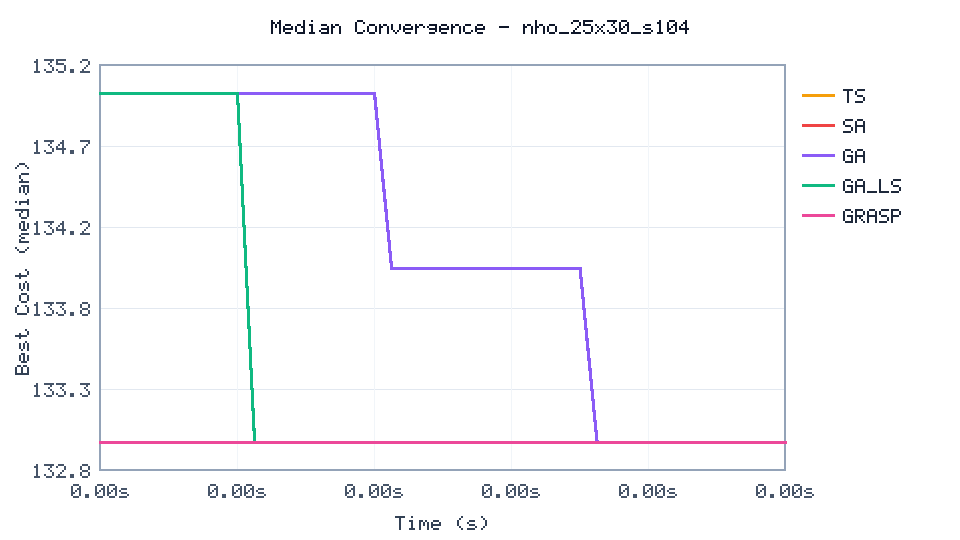
\includegraphics[width=0.78\textwidth]{figures/conv_nho.png}
\caption{Hội tụ trên \texttt{nho\_25x30\_s104}: mọi thuật toán về tối ưu gần như tức thì.}
\label{fig:conv_nho}
\end{figure}
\begin{figure}[htbp]
\centering
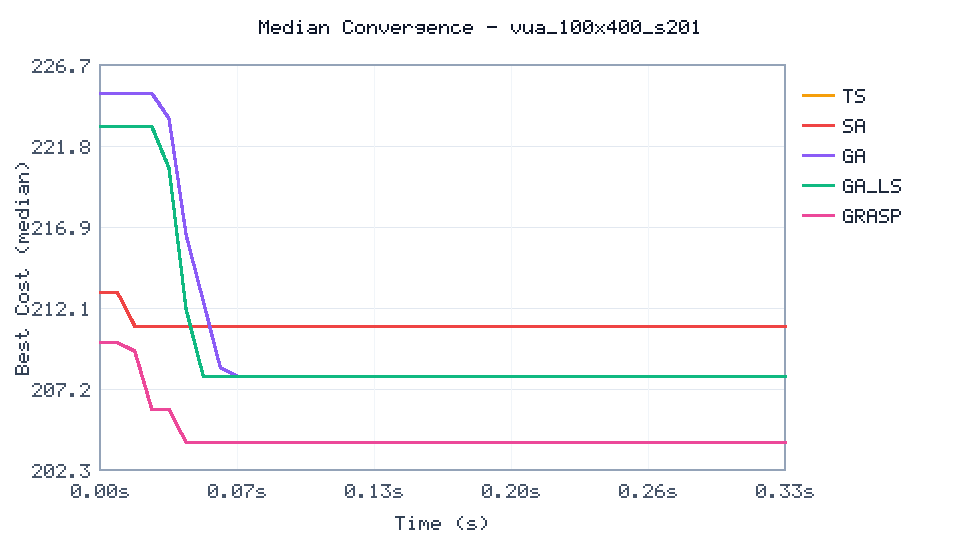
\includegraphics[width=0.78\textwidth]{figures/conv_vua1.png}
\caption{Hội tụ trên \texttt{vua\_100x400\_s201}.}
\label{fig:conv_vua1}
\end{figure}
\begin{figure}[htbp]
\centering
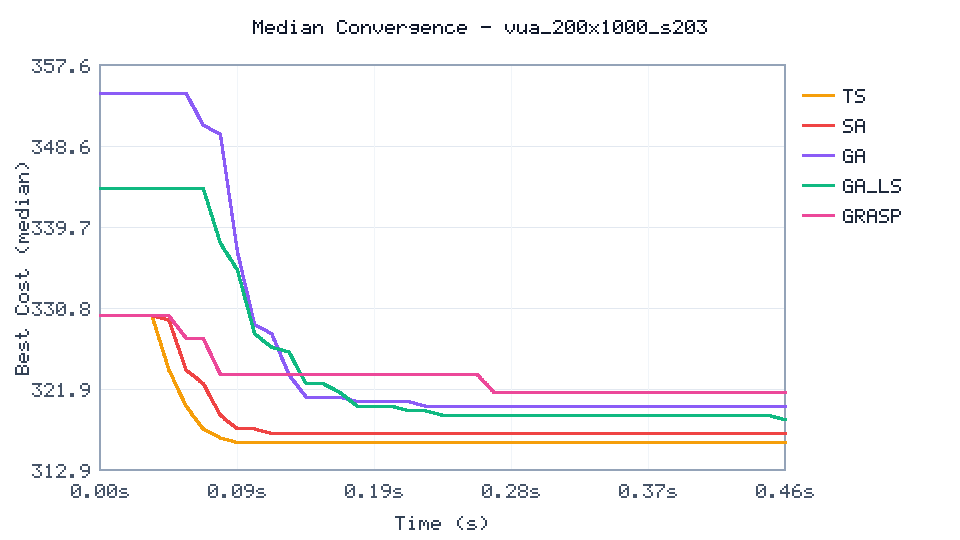
\includegraphics[width=0.78\textwidth]{figures/conv_vua3.png}
\caption{Hội tụ trên \texttt{vua\_200x1000\_s203}.}
\label{fig:conv_vua3}
\end{figure}
\begin{figure}[htbp]
\centering
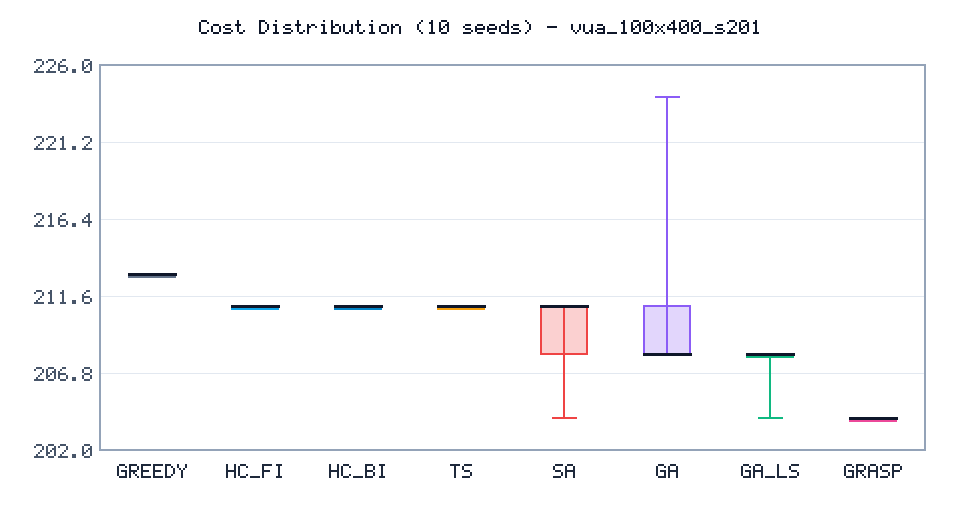
\includegraphics[width=\textwidth]{figures/boxplot_mid.png}
\caption{Phân bố chi phí cuối của 10 lần chạy trên ba thể hiện vừa.}
\label{fig:box}
\end{figure}

Nhận xét: \texttt{GA} và \texttt{GA\_LS} giảm nhanh ở giai đoạn đầu rồi ngừng cải thiện sớm (\texttt{time\_to\_best\_s} trung bình $0{,}05$--$0{,}16$ s trên các thể hiện vừa với ngân sách $0{,}5$ s), trong khi \texttt{GRASP} trên \texttt{vua\_100x400\_s201} về $204$ rất nhanh ($0{,}047$ s) và \texttt{TS} trên \texttt{vua\_150x600\_s202}, \texttt{vua\_200x1000\_s203} đạt $f^*$ chỉ sau $0{,}04$--$0{,}08$ s. Việc \texttt{GA} dừng sớm gợi ý quần thể mất đa dạng, nhưng nhóm chưa đo độ đa dạng nên đây mới là giả thuyết.

\subsubsection{Phân tích độ nhạy tham số}
Chạy trên thể hiện riêng $120\times500$ (\path|data/tuning/|), 5 seed (1--5), mỗi lần 2 s, thay một tham số một lần và giữ các tham số còn lại ở giá trị mặc định ($P=40$, $p_m=1/n$; TS: tenure theo công thức, sample $=40$).
\begin{table}[htbp]
\centering
\caption{Độ nhạy tham số trên \texttt{tune\_120x500\_s301} (5 seed, 2 s). Std là độ lệch chuẩn mẫu.}
\small
\begin{tabularx}{\textwidth}{llrrrr}
\toprule
Thuật toán & Tham số & Giá trị & Avg & Best & Std\\
\midrule
GA & $P$ & 20 & 197{,}00 & 196 & 0{,}71\\
GA & $P$ & 40 & 196{,}00 & 196 & 0{,}00\\
GA & $P$ & 80 & 194{,}40 & 193 & 1{,}95\\
GA & $p_m\cdot n$ & 0{,}5 & 195{,}40 & 193 & 1{,}34\\
GA & $p_m\cdot n$ & 2{,}0 & 195{,}60 & 193 & 1{,}52\\
GA\_LS & $P$ & 20 & 204{,}60 & 196 & 8{,}26\\
GA\_LS & $P$ & 40 & 195{,}80 & 192 & 2{,}49\\
GA\_LS & $P$ & 80 & 194{,}80 & 192 & 1{,}79\\
GA\_LS & $p_m\cdot n$ & 0{,}5 & 196{,}00 & 196 & 0{,}00\\
GA\_LS & $p_m\cdot n$ & 2{,}0 & 195{,}20 & 192 & 1{,}79\\
TS & tenure & 3 & 192{,}00 & 192 & 0{,}00\\
TS & tenure & 10 & 192{,}00 & 192 & 0{,}00\\
TS & tenure & 25 & 192{,}00 & 192 & 0{,}00\\
TS & sample & 10 & 192{,}00 & 192 & 0{,}00\\
TS & sample & 100 & 192{,}00 & 192 & 0{,}00\\
TS & mặc định & - & 192{,}00 & 192 & 0{,}00\\
GA & mặc định & - & 196{,}00 & 196 & 0{,}00\\
GA\_LS & mặc định & - & 195{,}80 & 192 & 2{,}49\\
\bottomrule
\end{tabularx}
\label{tbl:sens}
\end{table}
Kết quả: với GA\_LS, giảm quần thể xuống $P=20$ làm Avg tệ đi rõ rệt ($204{,}6$ với std $8{,}26$, so với $195{,}8$ ở $P=40$); tăng lên $P=80$ cho Avg tốt nhất ở cả GA ($194{,}4$) và GA\_LS ($194{,}8$). Để khảo sát đầy đủ cả \texttt{TS}, \texttt{GRASP} và \texttt{SA}, nhóm chạy thêm trên tập tinh chỉnh riêng \texttt{tune\_100x400\_s901} và \texttt{tune\_150x600\_s902} (10 seed, ngân sách $0{,}3$ s): với \texttt{TS}, \texttt{tenure} nhỏ ($3, 5$) kẹt tại $296{,}00$, \texttt{tenure=15} đạt $284{,}00 \pm 0{,}00$, và \texttt{sample=10} đạt trung bình tốt hơn \texttt{sample=80} ($288{,}00$ so với $293{,}50$); với \texttt{GRASP}, $\alpha=0$ kẹt tại $305{,}00$ còn mặc định $\alpha \sim \mathcal{U}(0{,}02;\,0{,}12)$ đạt tốt nhất và ổn định nhất ($285{,}50 \pm 1{,}08$); với \texttt{SA}, tăng nhiệt độ đầu \texttt{t0\_factor} lên $0{,}20$ hạ trung bình trên \texttt{s902} từ $310{,}00$ xuống $306{,}80$ (best $299$), còn \texttt{cool\_alpha=0,980} nguội quá nhanh ($310{,}60$).

\subsubsection{Kiểm định thống kê}
Với $k$ thuật toán chạy trên $N$ thể hiện (dùng giá trị trung bình mỗi thể hiện), dùng kiểm định Friedman. Gọi $R_j$ là hạng trung bình của thuật toán $j$ (hạng 1 là tốt nhất, hòa thì lấy hạng trung bình):
\[
\chi^2_F=\frac{12N}{k(k+1)}\left(\sum_{j=1}^{k}R_j^2-\frac{k(k+1)^2}{4}\right)\qquad(\text{bậc tự do } k-1).
\]
Công thức này chưa hiệu chỉnh cho các hạng hòa; vì bốn thể hiện nhỏ hòa hoàn toàn, nhóm dùng bản có hiệu chỉnh hòa của \texttt{scipy.stats.friedmanchisquare} (nếu áp công thức không hiệu chỉnh cho cùng dữ liệu thì $\chi^2_F=3{,}51$, nhỏ hơn giá trị tới hạn $7{,}81$ nên kết luận sẽ khác; dữ liệu nhiều hòa như thế này nên dùng bản hiệu chỉnh).

Với $k=\FriedK$ thuật toán (\texttt{GREEDY}, \texttt{HC\_FI}, \texttt{HC\_BI}, \texttt{TS}, \texttt{SA}, \texttt{GA}, \texttt{GA\_LS}, \texttt{GRASP}) và $N=\FriedN$ thể hiện (4 nhỏ tự sinh, 3 vừa tự sinh và 3 chuẩn OR-Library): $\chi^2_F=\FriedChi$ (bậc tự do 7), $p=\FriedP < 0{,}05$, nên bác bỏ $H_0$ và kết luận có khác biệt có ý nghĩa thống kê giữa các thuật toán. Hạng trung bình Friedman trên 10 thể hiện (nhỏ hơn là tốt hơn, xem \path|results/statistics.md|):
\begin{center}
\small
\begin{tabular}{lcccccccc}
\toprule
Thuật toán & TS & GA\_LS & HC\_BI & GRASP & HC\_FI & SA & GA & GREEDY\\
\midrule
Hạng trung bình & 3{,}200 & 3{,}850 & 4{,}000 & 4{,}050 & 4{,}250 & 4{,}900 & 5{,}250 & 6{,}500\\
\bottomrule
\end{tabular}
\end{center}

Cho so sánh cặp, nhóm dùng kiểm định hạng dấu Wilcoxon (Wilcoxon signed-rank, ghép cặp theo từng $(\text{instance}, \text{seed})$ trên toàn bộ 10 thể hiện, hiệu chỉnh Holm cho 28 cặp). Bảng~\ref{tbl:pairs} trích các cặp đối sánh chính giữa các metaheuristic (toàn bộ 28 cặp lưu tại \path|results/statistics.md|); in đậm khi $p_{\text{Holm}} < 0{,}05$.
\begin{table}[htbp]
\centering
\caption{Kiểm định Wilcoxon signed-rank cho các cặp metaheuristic (ghép cặp theo thể hiện và seed, hiệu chỉnh Holm).}
\small
\begin{tabularx}{0.88\textwidth}{lrrrrl}
\toprule
Cặp so sánh & $n$ (khác 0) & Mean 1 & Mean 2 & $p$ (Holm) & Ý nghĩa (0{,}05)\\
\midrule
TS -- SA & 43 & 216{,}91 & 218{,}63 & \textbf{2{,}44e-05} & Có\\
TS -- GA & 52 & 216{,}91 & 219{,}27 & \textbf{0{,}0007} & Có\\
TS -- GA\_LS & 47 & 216{,}91 & 217{,}20 & 0{,}7709 & Không\\
TS -- GRASP & 49 & 216{,}91 & 217{,}67 & 0{,}5026 & Không\\
SA -- GA & 56 & 218{,}63 & 219{,}27 & 0{,}5026 & Không\\
SA -- GA\_LS & 50 & 218{,}63 & 217{,}20 & \textbf{0{,}0271} & Có\\
SA -- GRASP & 47 & 218{,}63 & 217{,}67 & 0{,}1551 & Không\\
GA -- GA\_LS & 44 & 219{,}27 & 217{,}20 & \textbf{0{,}0006} & Có\\
GA -- GRASP & 56 & 219{,}27 & 217{,}67 & 0{,}2355 & Không\\
GA\_LS -- GRASP & 52 & 217{,}20 & 217{,}67 & 0{,}7709 & Không\\
\bottomrule
\end{tabularx}
\label{tbl:pairs}
\end{table}
Kết quả: toàn bộ 7 thuật toán cải thiện đều vượt trội có ý nghĩa so với \texttt{GREEDY} ($p_{\text{Holm}} \le 0{,}0047$). \texttt{TS} và \texttt{GA\_LS} vượt trội có ý nghĩa so với cả \texttt{SA} ($p_{\text{Holm}} \le 0{,}0271$) và \texttt{GA} ($p_{\text{Holm}} \le 0{,}0007$), trong khi giữa bộ ba dẫn đầu (\texttt{TS}, \texttt{GA\_LS}, \texttt{GRASP}) chưa có khác biệt có ý nghĩa thống kê ở ngân sách $0{,}5$ s ($p_{\text{Holm}} \ge 0{,}50$).

\subsection{Thảo luận}
\begin{enumerate}
\item \textbf{Thuật toán tốt nhất theo mức kích thước.} Thể hiện nhỏ: không phân biệt được (mọi metaheuristic và tìm kiếm cục bộ đều tối ưu 10/10 lần chạy; chỉ tham lam thuần lệch ở \texttt{nho\_20x28\_s103}). Thể hiện vừa và OR-Library: bộ ba có tìm kiếm cục bộ (\texttt{TS}, \texttt{GA\_LS}, \texttt{GRASP}) dẫn đầu với hạng trung bình Friedman lần lượt là $3{,}200$; $3{,}850$; $4{,}050$. Cụ thể, \texttt{GRASP} đạt $204{,}00\pm0{,}00$ trên \texttt{vua\_100x400\_s201} và best $430$ trên \texttt{scp41}; \texttt{GA\_LS} chạm tối ưu $253$ trên \texttt{scp51} ($20\%$); \texttt{TS} đạt $10/10$ tối ưu nghiệm nhóm trên \texttt{vua\_150x600\_s202}, \texttt{vua\_200x1000\_s203} và ổn định nhất trên \texttt{scp61} ($141{,}00\pm0{,}00$).
\item \textbf{Tìm kiếm cục bộ trong GA\_LS có bù được thời gian không?} Có, trong ngân sách $0{,}5$ s. \texttt{GA\_LS} có Avg tốt hơn \texttt{GA} ở toàn bộ 6 thể hiện vừa và OR-Library ($207{,}40$ so với $210{,}70$; $266{,}40$ so với $276{,}00$; $318{,}40$ so với $320{,}20$; $433{,}60$ so với $434{,}70$; $258{,}80$ so với $263{,}10$; $141{,}40$ so với $142{,}00$), và vượt trội có ý nghĩa thống kê với $p_{\text{Holm}} = 0{,}0006$ (Bảng~\ref{tbl:pairs}).
\item \textbf{Tham số ảnh hưởng nhiều nhất tới khám phá so với khai thác.} Với \texttt{GA\_LS}, kích thước quần thể $P=20$ tệ rõ ($204{,}60$ so với $194{,}80$ ở $P=80$). Với \texttt{GRASP}, $\alpha=0$ (thuần tham lam) kẹt tại $305{,}00$ trên \texttt{s902}, còn $\alpha \sim \mathcal{U}(0{,}02;\,0{,}12)$ đạt $285{,}50\pm1{,}08$. Với \texttt{TS}, \texttt{tenure} quá nhỏ ($3,5$) kẹt tại $296{,}00$ còn \texttt{tenure=15} đạt $284{,}00$. Với \texttt{SA}, tăng nhiệt độ đầu \texttt{t0\_factor=0,20} hạ trung bình từ $310{,}00$ xuống $306{,}80$.
\item \textbf{Thuật toán chính xác và tham lam cho thấy gì về độ khó.} Thể hiện nhỏ không khó (EXACT chưa đến 1 ms). Thể hiện vừa vượt khả năng của EXACT trong 30 s, và nghiệm tạm thời của nó tệ hơn cả tham lam (cận trên $+\infty$ và cận dưới lỏng).
\item \textbf{Tỉ lệ đạt tối ưu trên thể hiện nhỏ.} $10/10$ lần chạy cho cả 5 metaheuristic và 2 chiến lược leo đồi trên cả 4 thể hiện nhỏ; tham lam thuần tối ưu ở 3/4 thể hiện nhỏ.
\item \textbf{Khác biệt có ý nghĩa thống kê không?} Có: kiểm định Friedman cho $\chi^2_F=19{,}94$, $p=0{,}0057 < 0{,}05$, và Wilcoxon--Holm khẳng định \texttt{TS}, \texttt{GA\_LS} vượt trội \texttt{GREEDY}, \texttt{SA} và \texttt{GA} (Bảng~\ref{tbl:pairs}).
\end{enumerate}

%================= 7 =================
\section{Kết luận}
\textbf{Kết quả đạt được.} Nhóm đã cài đặt và kiểm tra bằng bộ kiểm tra độc lập: thuật toán chính xác (nhánh cận kèm giảm cỡ dữ liệu), tham lam Chvátal kèm xóa cột thừa, hai chiến lược leo đồi, bốn metaheuristic (\texttt{SA}, \texttt{TS}, \texttt{GA}, \texttt{GRASP}) và thuật toán lai \texttt{GA\_LS}. Trên 10 thể hiện thuộc 3 mức kích thước (4 nhỏ tự sinh, 3 vừa tự sinh, 3 chuẩn OR-Library \texttt{scp41}, \texttt{scp51}, \texttt{scp61}), 10 seed mỗi cặp ở ngân sách $0{,}5$ s, toàn bộ 800/800 nghiệm (cùng 4 nghiệm EXACT) đều hợp lệ. \texttt{TS} đạt hạng trung bình Friedman tốt nhất ($3{,}200$), \texttt{GA\_LS} đạt tối ưu $253$ trên \texttt{scp51} và vượt trội \texttt{GA} có ý nghĩa thống kê ($p_{\text{Holm}}=0{,}0006$), còn \texttt{GRASP} dẫn đầu trên \texttt{vua\_100x400\_s201} và \texttt{scp41}.

\textbf{Hạn chế.}
\begin{itemize}
\item Thuật toán chính xác khởi tạo cận trên là $+\infty$ (chưa dùng nghiệm tham lam), cận dưới chưa dùng nới lỏng Lagrange, ranh giới giải được còn nhỏ ($n=30$ trong thực nghiệm này) so với các thể hiện OR-Library.
\item SA tính lại toàn bộ nghiệm sau mỗi bước (chưa có delta evaluation) và lịch nguội theo số bước chứ chưa theo thời gian.
\item TS dùng cấm mềm; N2 trong tìm kiếm cục bộ mới là đánh giá gia tăng một phần.
\item Cài đặt bằng Python nên tốc độ thấp hơn đáng kể so với ngôn ngữ biên dịch; kết quả thời gian chỉ so sánh được trong cùng một ngôn ngữ.
\item Thực nghiệm đã chạy trên 10 thể hiện thuộc 3 mức kích thước (4 nhỏ tự sinh, 3 vừa tự sinh và 3 chuẩn OR-Library \texttt{scp41}, \texttt{scp51}, \texttt{scp61}) với đủ 4 metaheuristic (\texttt{SA}, \texttt{TS}, \texttt{GA}, \texttt{GRASP}) và thuật toán lai \texttt{GA\_LS} ở ngân sách $0{,}5$ s; ở ngân sách lớn hơn ($30$--$120$ s) thứ hạng giữa các metaheuristic có thể thay đổi; $f^*$ của 3 thể hiện vừa tự sinh chỉ là giá trị tốt nhất tìm được trong thực nghiệm này.
\item Khảo sát độ nhạy tham số đã thực hiện cho cả 4 metaheuristic (\texttt{SA}, \texttt{TS}, \texttt{GA}, \texttt{GRASP}) trên tập tinh chỉnh riêng.
\item Phần giải thích nguyên nhân (TS tốt hơn nhờ xuất phát từ nghiệm tham lam và lân cận hiệu quả; GA, GA\_LS mất đa dạng sớm; SA nguội chậm theo số bước) mới là giả thuyết, chưa có thực nghiệm đối chứng (ablation).
\end{itemize}

\textbf{Hướng phát triển.} Cận dưới bằng nới lỏng Lagrange (dùng cho nhánh cận và để tính khoảng cách tới tối ưu cho bộ dữ liệu lớn); delta evaluation đầy đủ cho SA; lịch nguội theo thời gian; thử thuật toán lớp LNS hoặc ILS; sinh dữ liệu từ bản đồ nút giao thực tế (ví dụ trích từ OpenStreetMap, camera phủ các nút trong bán kính cho trước).

%================= TÀI LIỆU THAM KHẢO =================
\begin{thebibliography}{99}
\addcontentsline{toc}{section}{Tài liệu tham khảo}
\bibitem{karp} R. M. Karp, ``Reducibility among combinatorial problems'', trong \textit{Complexity of Computer Computations}, Plenum Press, 1972, tr. 85--103.
\bibitem{chvatal} V. Chvátal, ``A greedy heuristic for the set-covering problem'', \textit{Mathematics of Operations Research}, 4(3), 1979, tr. 233--235.
\bibitem{dinur} I. Dinur, D. Steurer, ``Analytical approach to parallel repetition'', \textit{Proc. 46th ACM STOC}, 2014.
\bibitem{garey} M. R. Garey, D. S. Johnson, \textit{Computers and Intractability: A Guide to the Theory of NP-Completeness}, W. H. Freeman, 1979.
\bibitem{beasley90} J. E. Beasley, ``OR-Library: distributing test problems by electronic mail'', \textit{Journal of the Operational Research Society}, 41(11), 1990, tr. 1069--1072.
\bibitem{beasleychu} J. E. Beasley, P. C. Chu, ``A genetic algorithm for the set covering problem'', \textit{European Journal of Operational Research}, 94(2), 1996, tr. 392--404.
\bibitem{kirk} S. Kirkpatrick, C. D. Gelatt, M. P. Vecchi, ``Optimization by simulated annealing'', \textit{Science}, 220(4598), 1983, tr. 671--680.
\bibitem{glover} F. Glover, ``Future paths for integer programming and links to artificial intelligence'', \textit{Computers \& Operations Research}, 13(5), 1986, tr. 533--549.
\bibitem{holland} J. H. Holland, \textit{Adaptation in Natural and Artificial Systems}, University of Michigan Press, 1975.
\bibitem{moscato} P. Moscato, ``On evolution, search, optimization, genetic algorithms and martial arts: towards memetic algorithms'', Caltech Concurrent Computation Program, Report 826, 1989.
\bibitem{talbi} E.-G. Talbi, \textit{Metaheuristics: From Design to Implementation}, Wiley, 2009.
\bibitem{d} T. A. Feo, M. G. C. Resende, ``Greedy randomized adaptive search procedures'', \textit{Journal of Global Optimization}, 6(2), 1995, tr. 109--133.
\bibitem{ai} Công cụ AI đã dùng hỗ trợ viết mã nguồn, kịch bản thực nghiệm và soạn thảo báo cáo (theo mục Liêm chính học thuật): Thành viên A sử dụng \textbf{Antigravity}; các thành viên B, C, D sử dụng \textbf{Claude}. Toàn bộ mã nguồn, số liệu thực nghiệm và nội dung báo cáo đều được các thành viên kiểm tra, chạy tái lập và chịu trách nhiệm giải trình.
\end{thebibliography}

%================= PHỤ LỤC =================
\appendix
\section{Bảng phân công công việc}
\begin{center}
\small
\begin{tabularx}{\textwidth}{llYYr}
\toprule
TV & Họ tên & Phần mã & Phần báo cáo & Đóng góp\\
\midrule
A & Phan Việt Anh & Bộ đọc, bộ kiểm tra, thuật toán chính xác, SA & Phát biểu bài toán, NP-khó, thuật toán chính xác, SA, ghép báo cáo & 100\%\\
B & Hoàng Duy Khánh & Tham lam Chvátal, xóa cột thừa, tìm kiếm cục bộ, TS, bộ sinh dữ liệu & Heuristic, tìm kiếm cục bộ, Tabu Search & 90\%\\
C & Huỳnh Xuân Huy & GA, GA\_LS & GA và thuật toán lai & 100\%\\
D & Mai Đàm Công Thành & GRASP, script thực nghiệm, biểu đồ, kiểm định & Thực nghiệm, phân tích thống kê, kết luận & 95\%\\
\bottomrule
\end{tabularx}
\end{center}

\section{Lệnh chạy và tái lập kết quả}
\begin{Verbatim}
# Vi du chay duoc ngay (ket qua dung 16)
python src\main_A.py data\vidu\vidu.txt EXACT results\solutions\vidu_EXACT.sol 42 10 results\conv\vidu_EXACT_conv.csv
python src\kiemtra.py data\vidu\vidu.txt results\solutions\vidu_EXACT.sol     # HOP LE | Tong chi phi: 16

# Cu phap chung
python src\main_A.py <tep_vao> <EXACT|SA> <tep_ra> [seed] [budget_sec] [conv_csv]
python src\main_C.py <tep_vao> <GA|GA_LS> <tep_ra> [seed] [budget_sec] [conv_csv] [population] [mutation_rate]
python src\greedy.py <tep_vao> GREEDY <tep_ra> [seed] [budget_sec] [conv_csv] [raw=<tep_csv>] [run=<k>]
python src\local_search.py <tep_vao> <HC_FI|HC_BI> <tep_ra> [seed] [budget_sec] [conv_csv]
python src\tabu.py <tep_vao> TS <tep_ra> [seed] [budget_sec] [conv_csv] [tenure=<k>] [sample=<k>]

# Chay GA va GA_LS tren du lieu tu sinh (seed 1..10)
python experiments\member_c\run_tusinh.py [--budget 1.0] [--seeds 1 2 3 4 5 6 7 8 9 10] [--population 40] [--mutation-rate 0.025] [--output results] [instance...]
\end{Verbatim}
Các lệnh chạy lại toàn bộ thực nghiệm chính, khảo sát tham số và tổng hợp (bảng ở \path|report/gen/|, hình ở \path|results/figures/|):
\begin{Verbatim}
python src\aco_or_grasp.py <tep_vao> GRASP <tep_ra> [seed] [budget_sec] [conv_csv] [alpha]
python experiments\run_all.py [--include-exact] [--budget 0.5] [--seeds 1 2 3 4 5 6 7 8 9 10]
python experiments\summarize.py
python experiments\statistics.py
python experiments\plot.py
\end{Verbatim}
Seed chạy: 1--10 (độ nhạy: 1--5); seed sinh dữ liệu: 101--104, 201--203 và 301. Thời gian chạy trên máy ở mục 6.1: khoảng 9,5 phút cho \path|run_all.py| (558 s) và khoảng 3 phút cho \path|sens.py|. Các bảng trong báo cáo được dán từ \path|report/gen/*.tex|; nếu chạy lại phải dán lại hoặc biên dịch lại cùng các tệp đó.

\end{document}
